% P05 pilot best checkpoints; source-validation development fits, not outer-test results.
% data_sha256=068603f13027122fc53a26b4dc0ce4a146f397d5fb6276fb10ab60c4a6fcc0ff
\documentclass[tikz,border=8pt]{standalone}
\usepackage{pgfplots}
\pgfplotsset{compat=1.18}
\usepgfplotslibrary{groupplots}
\ifdefined\pdfinfoomitdate\pdfinfoomitdate=1\fi
\ifdefined\pdfsuppressptexinfo\pdfsuppressptexinfo=-1\fi
\ifdefined\pdftrailerid\pdftrailerid{}\fi
\definecolor{p05Dzero}{HTML}{0072B2}
\definecolor{p05Done}{HTML}{E69F00}
\definecolor{p05Dtwo}{HTML}{009E73}
\definecolor{p05Dthree}{HTML}{CC79A7}
\begin{document}
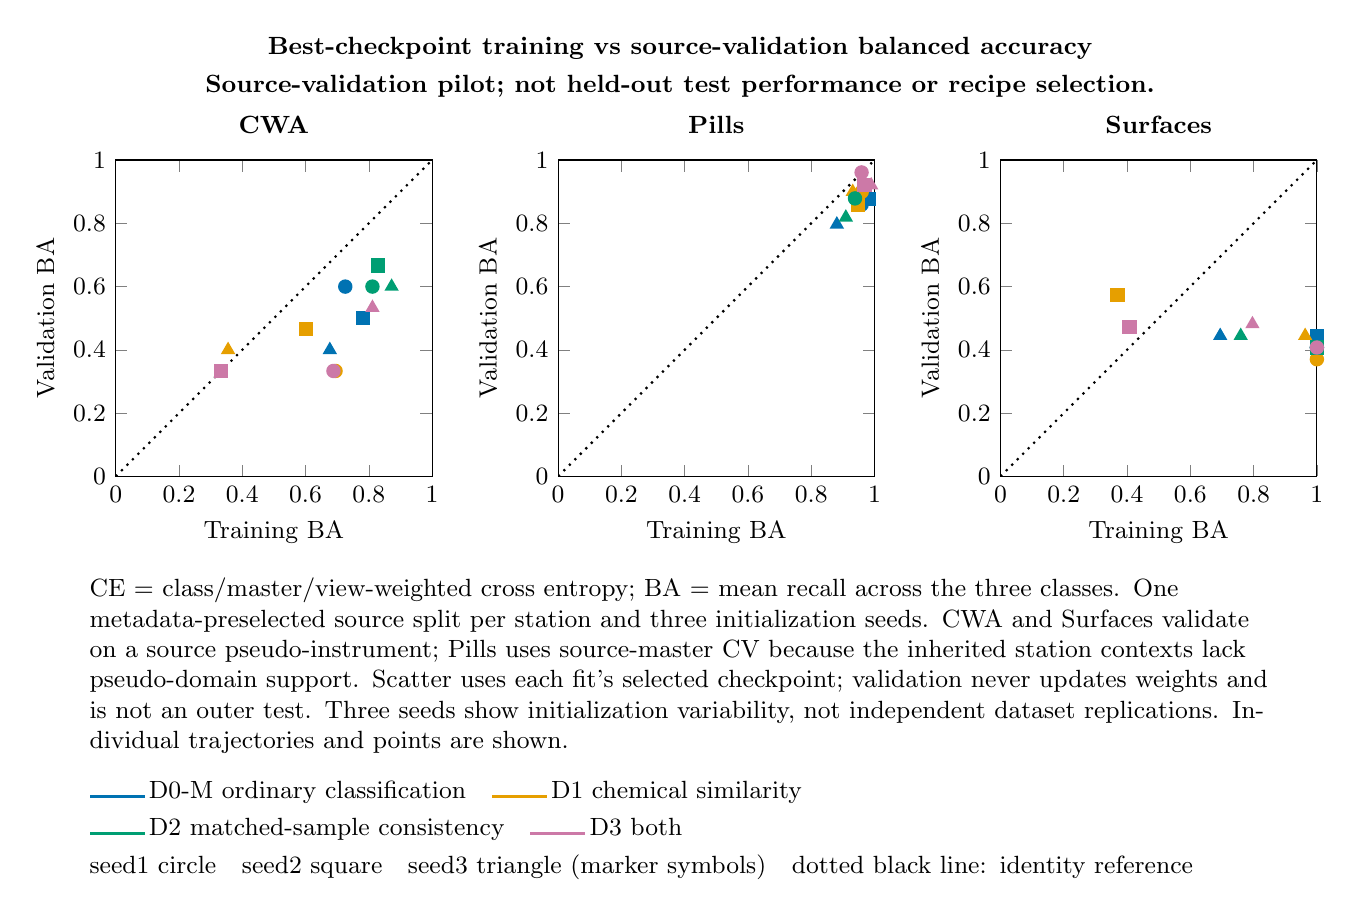
\begin{tikzpicture}
\begin{groupplot}[
  group style={group size=3 by 1, ylabels at=edge left, horizontal sep=1.6cm},
  width=5.6cm, height=5.6cm,
  every axis plot/.append style={line width=0.8pt},
  tick label style={font=\small, color=black},
  label style={font=\small, color=black},
  title style={font=\small\bfseries, color=black},
]
\nextgroupplot[title={CWA}, xlabel={Training BA}, ylabel={Validation BA}, xmin=0, xmax=1, ymin=0, ymax=1]
\addplot[black, dotted, line width=0.8pt, forget plot] coordinates {(0,0) (1,1)};
\addplot[only marks, color=p05Dzero, mark=*, mark size=2.2pt] coordinates {(0.72558922558922567,0.59999999999999998)};
\addplot[only marks, color=p05Dzero, mark=square*, mark size=2.2pt] coordinates {(0.78114478114478114,0.5)};
\addplot[only marks, color=p05Dzero, mark=triangle*, mark size=2.2pt] coordinates {(0.6767676767676768,0.39999999999999997)};
\addplot[only marks, color=p05Done, mark=*, mark size=2.2pt] coordinates {(0.69489769489769493,0.33333333333333331)};
\addplot[only marks, color=p05Done, mark=square*, mark size=2.2pt] coordinates {(0.60230510230510237,0.46666666666666662)};
\addplot[only marks, color=p05Done, mark=triangle*, mark size=2.2pt] coordinates {(0.35521885521885527,0.39999999999999997)};
\addplot[only marks, color=p05Dtwo, mark=*, mark size=2.2pt] coordinates {(0.81144781144781142,0.59999999999999998)};
\addplot[only marks, color=p05Dtwo, mark=square*, mark size=2.2pt] coordinates {(0.82996632996632991,0.66666666666666663)};
\addplot[only marks, color=p05Dtwo, mark=triangle*, mark size=2.2pt] coordinates {(0.87205387205387197,0.59999999999999998)};
\addplot[only marks, color=p05Dthree, mark=*, mark size=2.2pt] coordinates {(0.68816368816368823,0.33333333333333331)};
\addplot[only marks, color=p05Dthree, mark=square*, mark size=2.2pt] coordinates {(0.33333333333333331,0.33333333333333331)};
\addplot[only marks, color=p05Dthree, mark=triangle*, mark size=2.2pt] coordinates {(0.81144781144781142,0.53333333333333333)};
\nextgroupplot[title={Pills}, xlabel={Training BA}, ylabel={Validation BA}, xmin=0, xmax=1, ymin=0, ymax=1]
\addplot[black, dotted, line width=0.8pt, forget plot] coordinates {(0,0) (1,1)};
\addplot[only marks, color=p05Dzero, mark=*, mark size=2.2pt] coordinates {(0.95921963630296958,0.85906862745098034)};
\addplot[only marks, color=p05Dzero, mark=square*, mark size=2.2pt] coordinates {(0.98198198198198205,0.87745098039215685)};
\addplot[only marks, color=p05Dzero, mark=triangle*, mark size=2.2pt] coordinates {(0.88099557891224567,0.79656862745098034)};
\addplot[only marks, color=p05Done, mark=*, mark size=2.2pt] coordinates {(0.95974099099099097,0.89950980392156854)};
\addplot[only marks, color=p05Done, mark=square*, mark size=2.2pt] coordinates {(0.94880296963630295,0.85784313725490191)};
\addplot[only marks, color=p05Done, mark=triangle*, mark size=2.2pt] coordinates {(0.93119160827494163,0.89950980392156854)};
\addplot[only marks, color=p05Dtwo, mark=*, mark size=2.2pt] coordinates {(0.93838630296963632,0.87867647058823517)};
\addplot[only marks, color=p05Dtwo, mark=square*, mark size=2.2pt] coordinates {(0.9682286453119785,0.92156862745098034)};
\addplot[only marks, color=p05Dtwo, mark=triangle*, mark size=2.2pt] coordinates {(0.90943026359693035,0.81862745098039225)};
\addplot[only marks, color=p05Dthree, mark=*, mark size=2.2pt] coordinates {(0.95921963630296958,0.96078431372549022)};
\addplot[only marks, color=p05Dthree, mark=square*, mark size=2.2pt] coordinates {(0.9682286453119785,0.92156862745098034)};
\addplot[only marks, color=p05Dthree, mark=triangle*, mark size=2.2pt] coordinates {(0.98958333333333337,0.92034313725490191)};
\nextgroupplot[title={Surfaces}, xlabel={Training BA}, ylabel={Validation BA}, xmin=0, xmax=1, ymin=0, ymax=1]
\addplot[black, dotted, line width=0.8pt, forget plot] coordinates {(0,0) (1,1)};
\addplot[only marks, color=p05Dzero, mark=*, mark size=2.2pt] coordinates {(1,0.40740740740740744)};
\addplot[only marks, color=p05Dzero, mark=square*, mark size=2.2pt] coordinates {(1,0.44444444444444442)};
\addplot[only marks, color=p05Dzero, mark=triangle*, mark size=2.2pt] coordinates {(0.69444444444444431,0.44444444444444442)};
\addplot[only marks, color=p05Done, mark=*, mark size=2.2pt] coordinates {(1,0.37037037037037041)};
\addplot[only marks, color=p05Done, mark=square*, mark size=2.2pt] coordinates {(0.37037037037037041,0.57407407407407407)};
\addplot[only marks, color=p05Done, mark=triangle*, mark size=2.2pt] coordinates {(0.96296296296296291,0.44444444444444442)};
\addplot[only marks, color=p05Dtwo, mark=*, mark size=2.2pt] coordinates {(1,0.40740740740740744)};
\addplot[only marks, color=p05Dtwo, mark=square*, mark size=2.2pt] coordinates {(1,0.40740740740740744)};
\addplot[only marks, color=p05Dtwo, mark=triangle*, mark size=2.2pt] coordinates {(0.75925925925925919,0.44444444444444442)};
\addplot[only marks, color=p05Dthree, mark=*, mark size=2.2pt] coordinates {(1,0.40740740740740744)};
\addplot[only marks, color=p05Dthree, mark=square*, mark size=2.2pt] coordinates {(0.40740740740740744,0.47222222222222215)};
\addplot[only marks, color=p05Dthree, mark=triangle*, mark size=2.2pt] coordinates {(0.79629629629629628,0.48148148148148145)};
\end{groupplot}
\node[anchor=south, font=\bfseries\small, color=black, align=center, text width=15cm] at (current bounding box.north) {Best-checkpoint training vs source-validation balanced accuracy\\[1mm]Source-validation pilot; not held-out test performance or recipe selection.};
\node[anchor=north, font=\small, color=black, align=left, text width=15cm] (p05caption) at ([yshift=-2mm]current bounding box.south) {CE = class/master/view-weighted cross entropy; BA = mean recall across the three classes. One metadata-preselected source split per station and three initialization seeds. CWA and Surfaces validate on a source pseudo-instrument; Pills uses source-master CV because the inherited station contexts lack pseudo-domain support. Scatter uses each fit's selected checkpoint; validation never updates weights and is not an outer test. Three seeds show initialization variability, not independent dataset replications. Individual trajectories and points are shown.};
\node[anchor=north west, font=\small, color=black, align=left, text width=15cm] at ([yshift=-1mm]p05caption.south west) {\textcolor{p05Dzero}{\rule{7mm}{1.2pt}}\,D0-M ordinary classification\quad \textcolor{p05Done}{\rule{7mm}{1.2pt}}\,D1 chemical similarity\\[0.8mm]\textcolor{p05Dtwo}{\rule{7mm}{1.2pt}}\,D2 matched-sample consistency\quad \textcolor{p05Dthree}{\rule{7mm}{1.2pt}}\,D3 both\\[1mm]seed1 circle\quad seed2 square\quad seed3 triangle (marker symbols)\quad dotted black line: identity reference};
\end{tikzpicture}
\end{document}
